\documentclass[tikz, border=1mm]{standalone}
\begin{document}
    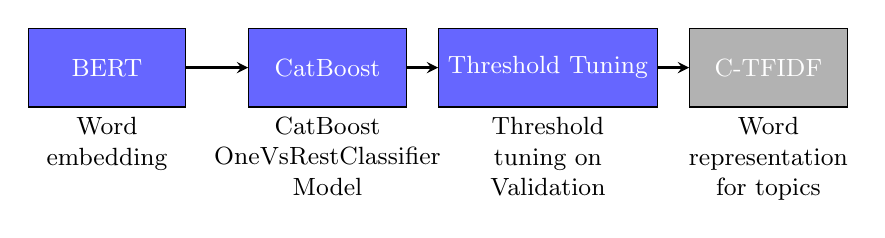
\begin{tikzpicture}[node distance=2.8cm, every node/.style={font=\small}]
    % Styles
    \tikzstyle{method} = [rectangle, minimum width=2cm, minimum height=1cm, text centered, draw=black, fill=blue!60, text=white]
    \tikzstyle{arrow} = [thick,->,>=stealth]
    \tikzstyle{caption} = [below, align=center]

    % Nodes
    \node (bert)   [method] {BERT};
    \node (catboost)   [method, right of=bert] {CatBoost};
    \node (trshld) [method, right of=catboost] {Threshold Tuning};
    \node (ctfidf) [method, right of=trshld, fill=gray!60] {C-TFIDF};

    % Arrows
    \draw [arrow] (bert) -- (catboost);
    \draw [arrow] (catboost) -- (trshld);
    \draw [arrow] (trshld) -- (ctfidf);

    % Captions
    \node [caption] at (bert.south)   {Word\\embedding};
    \node [caption] at (catboost.south)   {CatBoost\\OneVsRestClassifier\\Model};
    \node [caption] at (trshld.south) {Threshold\\tuning on\\Validation};
    \node [caption] at (ctfidf.south) {Word\\representation\\for topics};
    \end{tikzpicture}
\end{document}